\documentclass{article}
\usepackage[utf8]{inputenc}
\usepackage{amsmath,
	amssymb,
	datetime,
	hyperref,
	cleveref,
	mathtools,
	bbm,
	%mathabx,
	array,
	booktabs,
	xspace,
	calc,
	colortbl,
	siunitx,
	url,
 	graphicx}
\usepackage[dvipsnames]{xcolor}
\usepackage[giveninits=false,backend=biber,style=nature, maxcitenames =10, mincitenames=9]{biblatex}
\addbibresource{FJHown23.bib}
\addbibresource{FJH23.bib}
\title{QMC Blog Posts}
\author{QMCPy Crew}
\date{April 2020}
\input FJHDef.tex

\newcommand{\blogpost}[3]{\newpage%
\section{#1}%
\begin{refsection}%
	Authors(s): #2 and the QMCPy Team\bigskip #3%
\printbibliography[heading=subbibliography]
\end{refsection}
} %This command provides a new section and bibliography for each blogpost

\newcommand{\myshade}{60}
\colorlet{mylinkcolor}{violet}
\colorlet{mycitecolor}{violet}
\colorlet{myurlcolor}{YellowOrange}

\hypersetup{
	linkcolor  = mylinkcolor!\myshade!black,
	citecolor  = mycitecolor!\myshade!black,
	urlcolor   = myurlcolor!\myshade!black,
	colorlinks = true,
}

\newcommand{\FredComment}[1]{{\color{blue} Fred: #1}}
\newcommand{\AGSComment}[1]{{\color{green} Aleksei: #1}}
\newcommand{\SCComment}[1]{{\color{red} Sou-Cheng: #1}}
\newcommand{\MikeComment}[1]{{\color{orange} Mike: #1}}
\newcommand{\JagsComment}[1]{{\color{violet} Jags: #1}}


\begin{document}

\maketitle

\setcounter{tocdepth}{1}
\tableofcontents

\section{Introduction}
\FredComment{Comment}

We will be using this to construct and edit blog content for the launch of QMCPy.

Fred prefers to have each blog focus on just one idea, short and sweet.

The Google doc where we are defining the launch concept around the blogs is here \url{https://docs.google.com/document/d/1DcDdmwdUDCNKxGwUWCyQUjkTuQjhn-dskajlnEq14bo/edit?usp=sharing}

\section{Post 1: Intro to MC and why QMC is significant}

\blogpost{Why Add Q to MC?}{Fred Hickernell}{\label{WhyQ}

Quasi-Monte Carlo (QMC) methods can sometimes speed up simple Monte Carlo (MC) calculations by orders of magnitude?  What makes them work so well?

MC methods use computer generated random numbers to generate various scenarios.  When computing financial risk, the scenarios may be the possible market profit or losses under unknown future market conditions.  When assessing the resiliency of the power grid, the scenarios represent possible power demand and power grid failures under unknown future weather conditions.

If $Y$ is the quantity of interest, e.g., profit (or loss) one month from now, and $Y_1, \ldots, Y_n$ are its possible values under the model generating reasonable scenarios, then these computer generated data can be used to estimate the \emph{mean} or average quantity of interest, 
\[
\mu = \Ex(Y) \approx \frac 1n \bigl ( Y_1 + \cdots + Y_n \bigr) = \hmu_n.
\]
We are using a mean based on $n$ scenarios to approximate the true mean, which is based on an infinite number of scenarios.

Simple MC chooses $Y_1, \ldots, Y_n$ to be independent and identically distributed (IID).  Intuitively, this means that any $Y_i$ is chosen with no relationship to the other and all $Y_i$ come from the same probability distribution or model that generates the scenarios.

While this is a good idea, we can do better.  By choosing $Y_1, \ldots, Y_n$ to be more representative of the infinite number of possible scenarios, we can make $\hmu$ a better estimate of the mean.

The model that generates $Y$ is often written as $Y= f(\vX)$, where $\vX$ is a uniformly distributed vector in the $d$-dimensional unit cube $[0,1]^d$.  If $Y_i = f(\vX_i)$ for IID $\vX_i$, then we have simple MC.  Figure \ref{fig:iid_pts} shows a picture of IID uniform  $\vX_1, \ldots, \vX_{64}$ in $2$ dimensions.  Because the points are IID, there are gaps and clusters.

\begin{figure}[ht!]
    \centering
    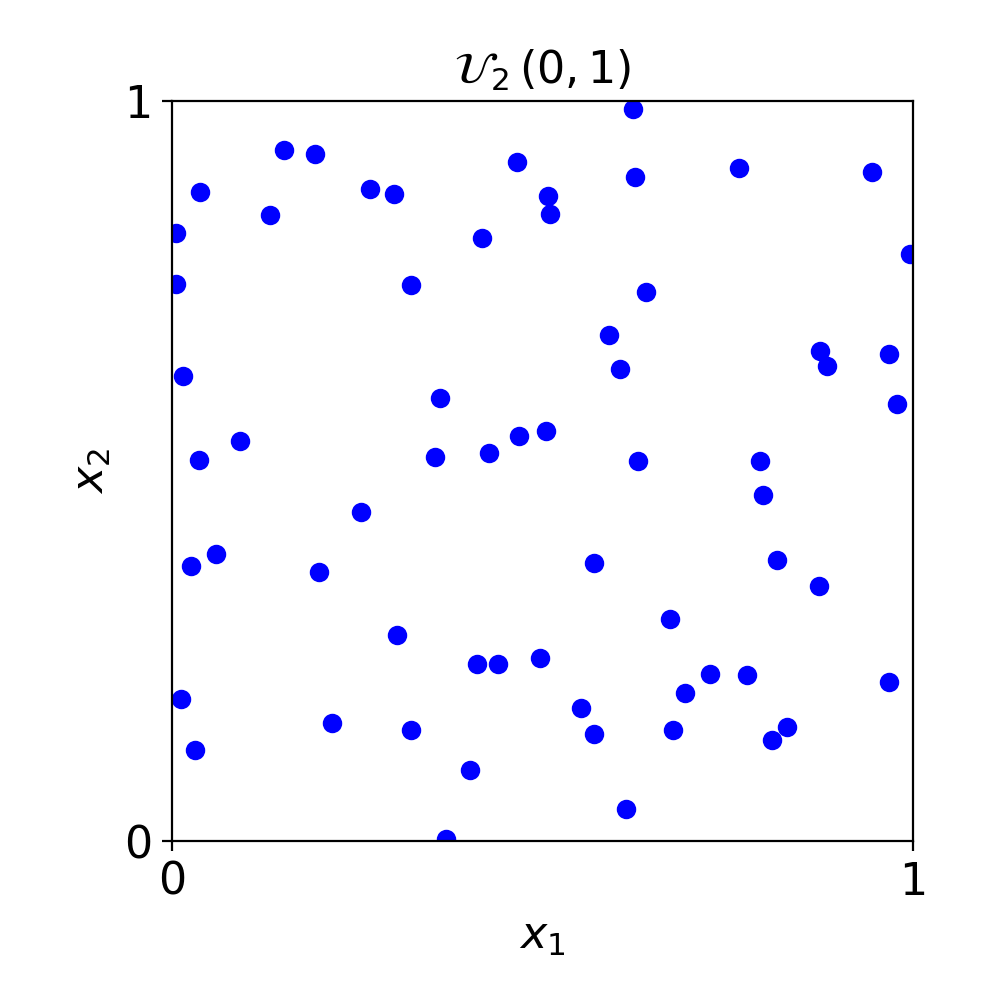
\includegraphics[width=.6\textwidth]{figures/iid_uniform_pts.png}
    \caption{64 IID standard uniform points in 2 dimensions.}
    \label{fig:iid_pts}
\end{figure}

Figure \ref{fig:lat_pts} gives an example of $\vX_1, \ldots, \vX_{64}$ used in QMC methods.  These points are called integration lattice points.  Note that they more evenly fill the square than the IID points in Figure \ref{fig:iid_pts}.

\begin{figure}[ht!]
    \centering
    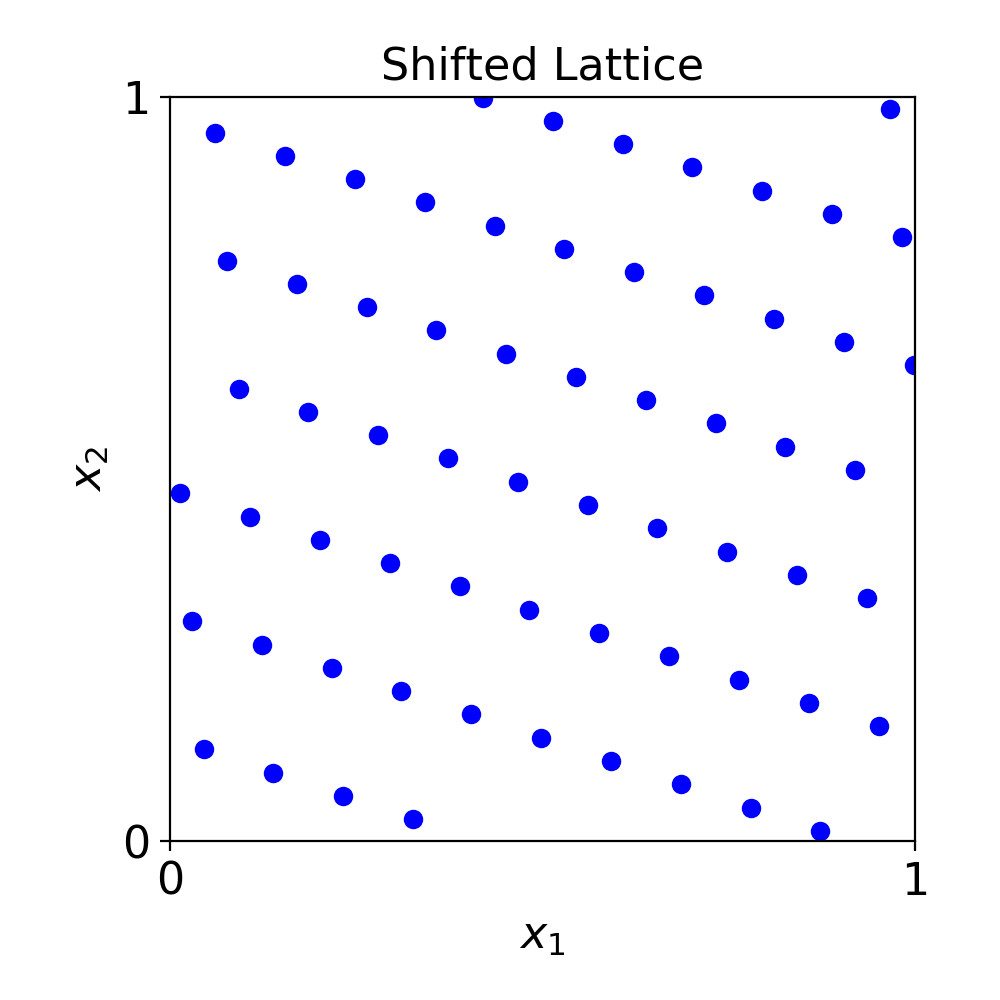
\includegraphics[width=.6\textwidth]{figures/lattice_pts.png}
    \caption{64 shifted lattice points in 2 dimensions.}
    \label{fig:lat_pts}
\end{figure}

Because these QMC points  are more even, they can give $\hmu_n$ with an error of nearly $\Order(n^{-1})$.  In contrast, the error of simple MC $\hmu_n$ is typically $\Order(n^{-1/2})$.  That's the reason to add Q to MC.

QMCPy \cite{QMCPy2020a} is our open source Python library that implements QMC methods, including point generators, cubatures, and stopping criteria.  This blog will introduce you to QMC and QMCPy.
}

\blogpost{A QMCPy Quick Start}{Sou-Cheng Choi, Aleksei Sorokin}{}

\blogpost{What Makes a Sequence ``Low Discrepancy"?}{}{}

\blogpost{A Brief History of Quasi-Monte Carlo}{}{}

\blogpost{Be Careful Replacing IID Sequences by Low Discrepancy Sequences}{}{}

\blogpost{Randomizing Your Low Discrepancy Points Helps}{}{}

\blogpost{What to Do when the Dimension is Infinite}{}{}

\blogpost{Variation/Variance Reduction for QMC}{}{}

\blogpost{When QMC Does Not Help}{}{}


\end{document}
